\section{Preempt RT}

\begin{frame}
  \frametitle{The PREEMPT\_RT Patch}
	\begin{itemize}
		\item One way to implement a multi-task Real-Time Operating System is to have a preemptible system
		\item Any task can be interrupted at any point so that higher priority tasks can run
		\item Userspace preemption already exists in Linux
		\item The Linux Kernel also supports real-time scheduling policies
		\item However, code that runs in kernel mode isn't fully preemptible
		\item The Preempt-RT patch aims at making all code running in kernel mode preemptible
	\end{itemize}
\end{frame}

\begin{frame}
  \frametitle{PREEMPT\_RT mainlining status (1)}
  \begin{itemize}
  \item The project is making good progress since it got funding from
        the Linux Foundation in 2015 (Linux version 4.1 at that time).
  \item We can now observe a slow but steady reduction of the size of
        the PREEMPT\_RT patchset:\\
    \vfill
    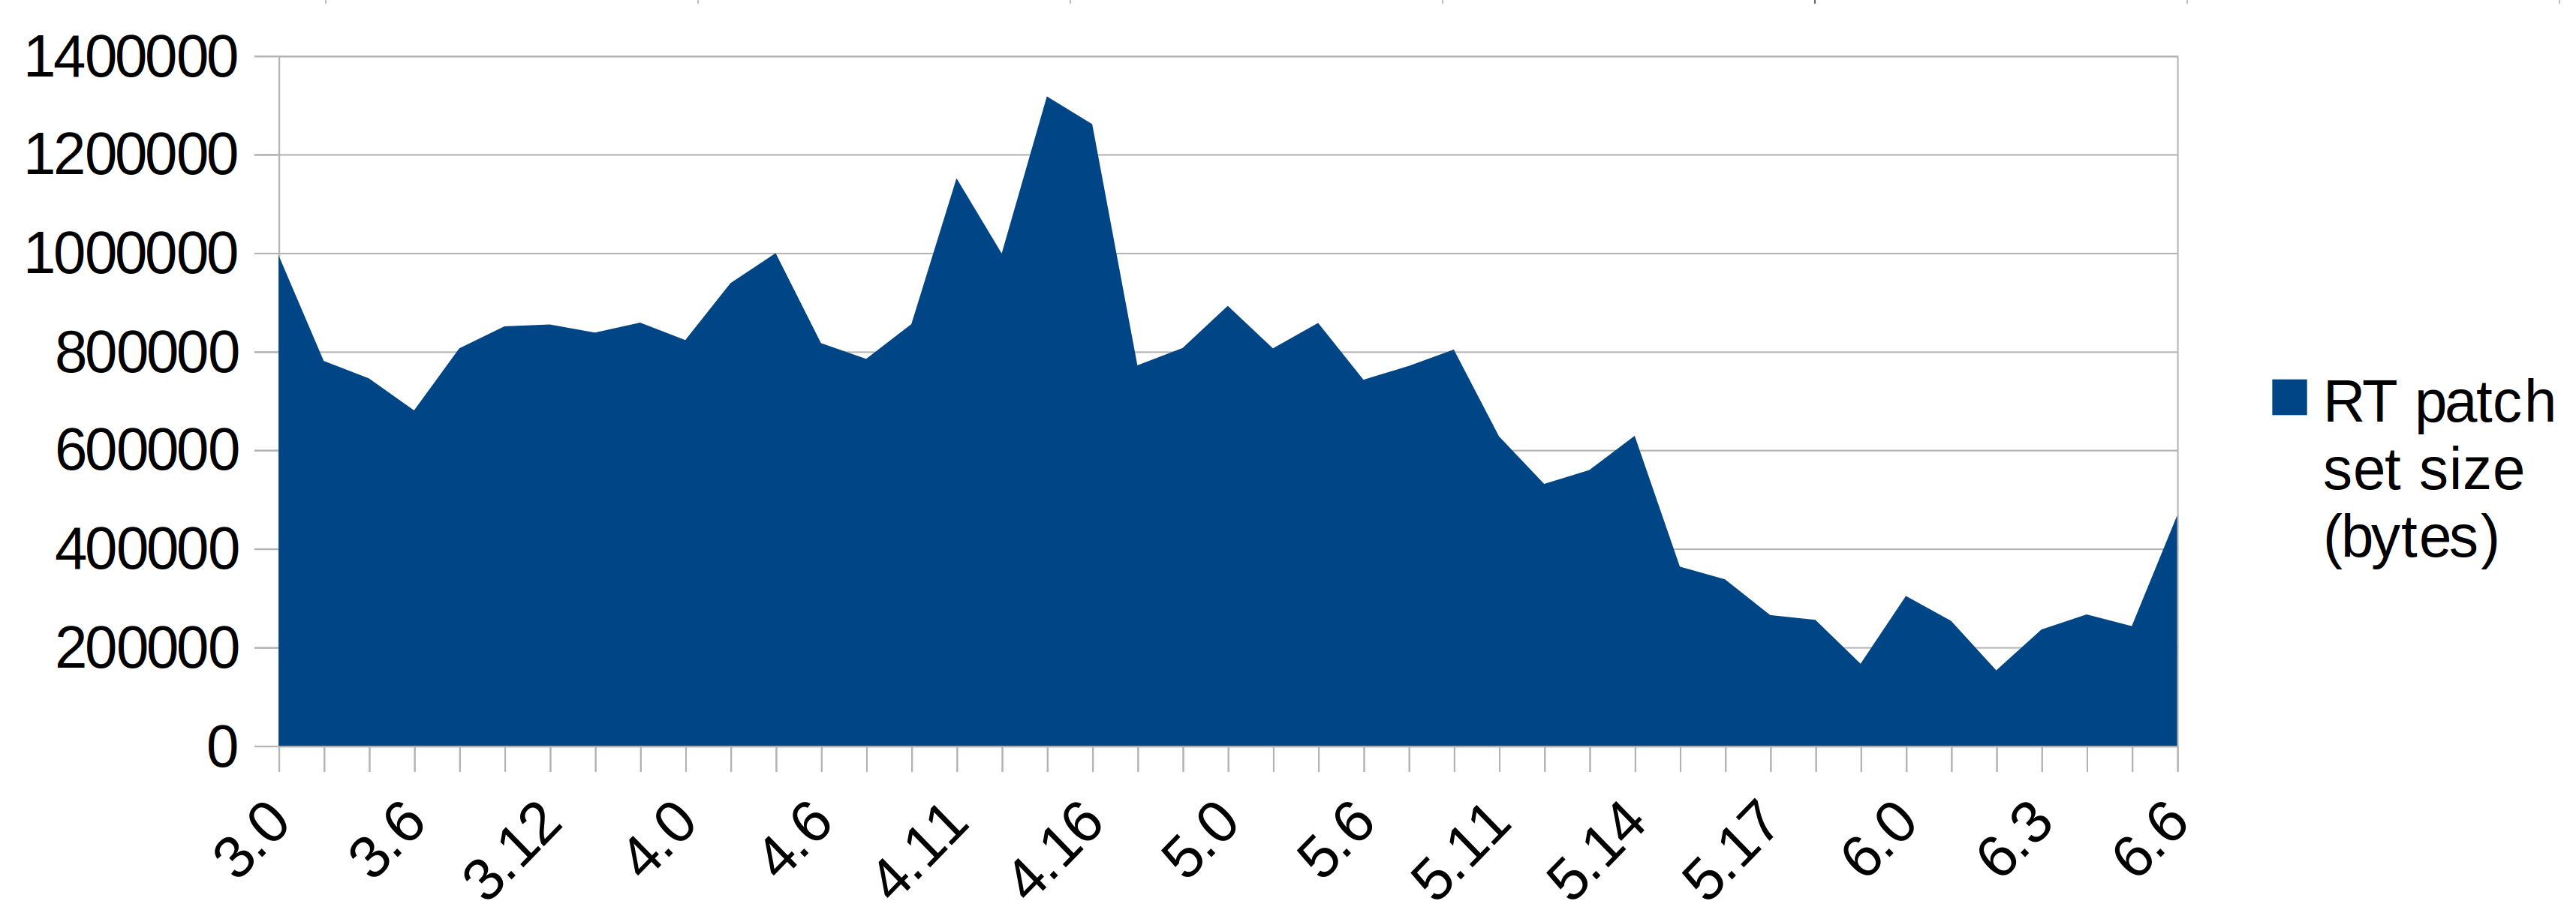
\includegraphics[width=0.8\textwidth]{slides/realtime-linux-preempt-rt/rt-patch-sizes.png}
  \end{itemize}
\end{frame}

\begin{frame}
  \frametitle{PREEMPT\_RT mainlining status (2)}
  \begin{itemize}
  \item However, the mainline Linux kernel is a moving target too,
        introducing new issues for real-time (such as disabling preemption in
        BPF... see \url{https://lwn.net/Articles/802884/}).
  \item In 5.12, new \kconfig{CONFIG_PREEMPT_DYNAMIC} switch to change the preemption
        model at boot time: \code{preempt=none}, \code{preempt=voluntary} or
        \code{preempt=full}
  \item In 5.15, the realtime preemption locking core is merged in mainline.
	This was the biggest part to mainline. A few pending changes are
	still left. See \url{https://lwn.net/Articles/867919/}.
  \item \code{printk()} is one of the remaining pieces to be upstreamed
  \item See the latest news on \url{https://wiki.linuxfoundation.org/realtime/}
  \end{itemize}
\end{frame}

\begin{frame}
	\frametitle{Why use PREEMPT\_RT ?}
	\begin{itemize}
		\item Allow using the POSIX/Linux API, which is portable and familiar
		\item Benefit from the huge hardware support provided by Linux
		\item Run common software in non-RT mode, and custom critical software in parallel
		\item Benefit from the community support and help
	\end{itemize}
\end{frame}

\begin{frame}
	\frametitle{Why not to use PREEMPT\_RT ?}
	\begin{itemize}
		\item Linux will never be a formally proven RTOS
		\item The hardware Linux tipycally runs on isn't designed with RT in mind
		\item The RT patch makes the Kernel deterministic and preemptible...
		\item ... but the goal is not to have the lowest latencies possible
		\item Linux will never be suitable for safety critical applications
	\end{itemize}
\end{frame}

\begin{frame}
  \frametitle{Getting the patch}
	\begin{itemize}
		\item The RT Patchset is released \textbf{every other} kernel release
		\item It can be gotten as a set of patches or a single patch : \\
			\url{https://cdn.kernel.org/pub/linux/kernel/projects/rt/}
		\item Kernel trees with the patch applied are also available :
			\begin{itemize}
				\item \url{http://git.kernel.org/cgit/linux/kernel/git/rt/linux-rt-devel.git}
				\item \url{http://git.kernel.org/cgit/linux/kernel/git/rt/linux-stable-rt.git}
			\end{itemize}
		\item Most build-systems like Buildroot or Yocto Project support building a RT Kernel
	\end{itemize}
\end{frame}

\begin{frame}
  \frametitle{The legacy of the RT patch}
  Many current features in the Linux Kernel originated from the RT patch :
	\begin{itemize}
		\item Kernel-side preemption
		\item High Resolution Timers
		\item Threaded interrupts
		\item Priority-Inheritance support for locking primitives
		\item Tickless operation
		\item Earliest-Deadline First scheduler
		\item Realtime locks - Locking primitives conversion
	\end{itemize}
\end{frame}


\begin{frame}
  \frametitle{Locking}
	\begin{itemize}
		\item Locks are synchronisation primitives that arbitrate concurrent accesses to a resource
		\item Several locking primitives exists in the Kernel and in Userspace
		\item Kernel lock families are :
			\begin{itemize}
				\item Sleeping locks
				\item CPU Local locks
				\item Spinning locks
			\end{itemize}
	\end{itemize}
\end{frame}

\begin{frame}
	\frametitle{Critical sections}
	\begin{itemize}
		\item Spinning locks can be taken with interrupts constraints
		\item Spinlock functions have variants with some suffixes :
		\begin{itemize}
		\item \code{_bh()}
			\begin{itemize}
				\item Disable / Enable soft interrupts (bottom halves)
			\end{itemize}
		\item \code{_irq()}
			\begin{itemize}
				\item Disable / Enable interrupts
			\end{itemize}
		\item \code{_irqsave()} / \code{_irqrestore()}
			\begin{itemize}
				\item Save and disable or restore interrupt state (if previously disabled)
			\end{itemize}
		\end{itemize}
		\item Dedicated functions also exist, but should be used only for the Kernel core
		\item \code{preempt_disable()} / \code{preempt_enable()}
			\begin{itemize}
				\item Disable / Enable preemption, to protect per-CPU data
			\end{itemize}
		\item \code{migrate_disable()} / \code{migrate_enable()}
			\begin{itemize}
				\item Disable / Enable migration, also to protect per-CPU data
			\end{itemize}

	\end{itemize}
\end{frame}

\begin{frame}
  \frametitle{Sleeping locks}
	\begin{itemize}
		\item Sleeping locks will sleep and schedule while waiting
		\item There are several types of sleeping locks :
	\begin{itemize}
		\item mutex
		\item rt\_mutex
		\item semaphore
		\item rw\_semaphore
	\end{itemize}
	\end{itemize}
\end{frame}

\begin{frame}
  \frametitle{Spinlocks}
  	\begin{itemize}
		\item Spinlocks will busy-wait until the lock is freed
		\item There exists several types of spinlocks :
		\begin{itemize}
			\item spinlock\_t
			\item rwlock\_t
			\item raw\_spinlock\_t
		\end{itemize}
		\item Spinlocks will disable preemption when taken
		\item With PREEMPT\_RT, \code{spinlock_t} and \code{rwlock_t} will become sleeping locks
	\end{itemize}
\end{frame}

\begin{frame}
  \frametitle{High resolution timers}
  \begin{itemize}
  \item The resolution of the timers used to be bound to the
    resolution of the regular system tick
    \begin{itemize}
    \item Usually 100 Hz or 250 Hz, depending on the architecture and
      the configuration
    \item A resolution of only 10 ms or 4 ms.
    \item Increasing the regular system tick frequency is not an
      option as it would consume too many resources
    \end{itemize}
  \item The high-resolution timers infrastructure allows to use
    the available hardware timers to program interrupts
    at the right moment.
    \begin{itemize}
    \item Hardware timers are multiplexed, so that a single hardware
      timer is sufficient to handle a large number of
      software-programmed timers.
    \item Usable directly from user space using the usual timer APIs
    \end{itemize}
  \end{itemize}
\end{frame}

\begin{frame}
  \frametitle{Printk}
	\begin{itemize}
		\item \code{printk()} is one of the main logging mechanism in the kernel
		\item It works in all execution context
		\item It's currently one of the last items preventing the RT-patch from being fully upstream
		\item Currently, the last kernel task who printed must print the full buffer
		\item A low priority task can block a high priority task by printing lots of data
		\item A low log-level can help remove these issues for now
	\end{itemize}
\end{frame}

\begin{frame}
  \frametitle{Interrupt handlers}
	\begin{itemize}
		\item Interrupt handlers run with interrupts disabled
		\item In PREEMPT\_RT, almost all interrupt handlers are \textbf{threaded}
		\item Very small hardware interrupt handlers are used, that have a well-defined execution time
		\item They acknowledge the interrupts, and enqueues the "real" interrupt handler
		\item The interrupt handler runs in a dedicated Kernel thread
		\item Threaded interrupts are well established in the mainline kernel
	\end{itemize}
%  https://wiki.linuxfoundation.org/realtime/documentation/technical_details/threadirq
\end{frame}

\begin{frame}
	\frametitle{Hard interrupts vs. Threaded interrupts}

	\begin{columns}
	\begin{column}{0.50\textwidth}
	\vspace{-1cm}
	\begin{figure}
	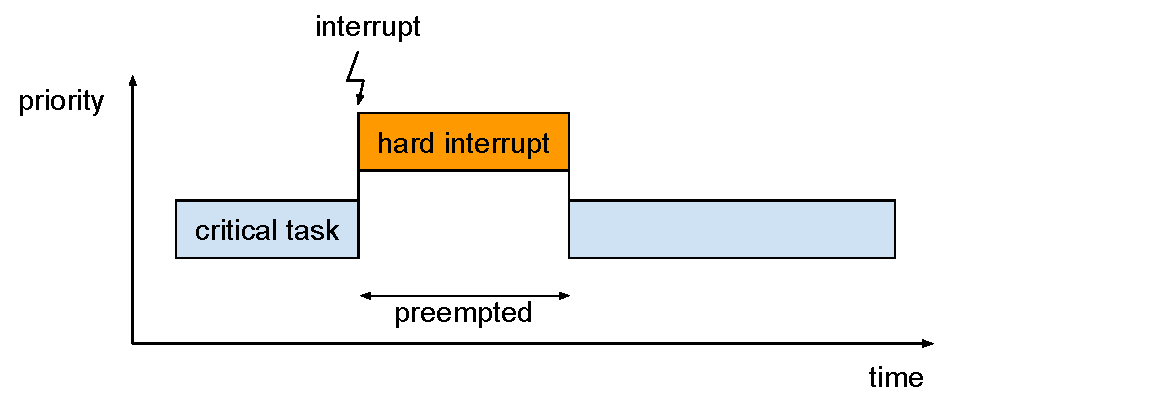
\includegraphics[height=0.35\textheight]{slides/realtime-linux-realtime-systems/irq_preemption.pdf}
	\vspace{-1cm}
	\caption{Hardware interrupt processing}
	\end{figure}
	\vspace{-0.6cm}
	\begin{figure}
	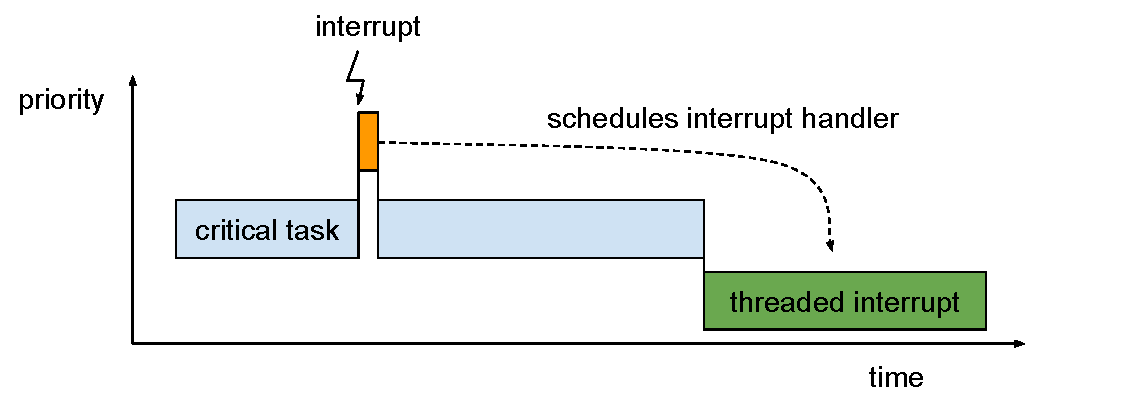
\includegraphics[height=0.35\textheight]{slides/realtime-linux-preempt-rt/softirq_preemption.pdf}
	\vspace{-0.8cm}
	\caption{Threaded interrupt processing}
	\end{figure}
	\end{column}

		\begin{column}{0.50\textwidth}
			\begin{itemize}
				\item Small, well-defined hard irq handlers
				\item Irq handlers run in a dedicated task
				\item It has a PID, and can be assigned a priority
				\item Critical tasks can run regardless of interrupts
				\item Use \code{ps -e} to list tasks
				\item Use \code{chrt -p <prio> <pid>} to change the priority
			\end{itemize}
		\end{column}
	\end{columns}
\end{frame}

\begin{frame}
  \frametitle{Uncompatible options}
	\begin{itemize}
		\item Some configuration options don't play well with realtime
		\item \code{CONFIG_LOCKUP_DETECTOR and CONFIG_DETECT_HUNG_TASK}
			\begin{itemize}
				\item Kernel tasks with a priority of 99, can introduce latencies
			\end{itemize}
		\item \code{CONFIG_DEBUG_*}
			\begin{itemize}
				\item Debugging options are very useful
				\item Most of them introduce latencies due to heavy logging
				\item Some options adds security checks and verifiers (lockdep)
			\end{itemize}
	\end{itemize}
\end{frame}

\begin{frame}
  \frametitle{Preemption models}
  The Linux kernel Scheduler has several preemption models available :
	\begin{itemize}
		\item PREEMPT\_NONE - No Forced Preemption (server)
		\item PREEMPT\_VOLUNTARY - Voluntary Kernel Preemption (Desktop)
		\item PREEMPT - Preemptible Kernel (Low-latency Desktop)
		\item PREEMPT\_RT - Fully Preemptible Kernel (Real-Time)
	\end{itemize}
\end{frame}

\begin{frame}
  \frametitle{1st option: no forced preemption}
  \kconfig{CONFIG_PREEMPT_NONE}\\
  Kernel code (interrupts, exceptions, system calls) never preempted.
  Default behavior in standard kernels.
  \begin{itemize}
  \item Best for systems making intense computations, on which overall
    throughput is key.
  \item Best to reduce task switching to maximize CPU and cache usage
    (by reducing context switching).
  \item Still benefits from some Linux real-time improvements: O(1)
    scheduler, increased multiprocessor safety (work on RT preemption
    was useful to identify hard to find SMP bugs).
  \item Can also benefit from a lower timer frequency (several possible
        values between 100 Hz and 1000 Hz).
  \end{itemize}
\end{frame}

\begin{frame}
  \frametitle{2nd option: voluntary kernel preemption}
  \kconfig{CONFIG_PREEMPT_VOLUNTARY}\\
  Kernel code can preempt itself
  \begin{itemize}
  \item Typically for desktop systems, for quicker application
    reaction to user input.
  \item Adds explicit rescheduling points (\kfunc{might_sleep})
        throughout kernel code.
  \item Minor impact on throughput.
  \item Still used in: Ubuntu Desktop 20.04
  \end{itemize}
\end{frame}

\begin{frame}
  \frametitle{3rd option: preemptible kernel}
  \kconfig{CONFIG_PREEMPT}\\
  Most kernel code can be involuntarily preempted at any time.  When a
  process becomes runnable, no more need to wait for kernel code
  (typically a system call) to return before running the scheduler.
  \begin{itemize}
  \item Exception: kernel critical sections (holding spinlocks):
  \begin{center}
    \includegraphics[width=0.9\textwidth]{common/spinlock-deadlock-with-preemption.pdf}
  \end{center}
  \item Typically for desktop or embedded systems with latency
    requirements in the milliseconds range. Still a relatively minor impact on throughput.
  \end{itemize}
\end{frame}

\begin{frame}
	\frametitle{4th option: fully preemptible kernel}
	  \kconfig{CONFIG_PREEMPT_RT}\\
	  Almost all kernel code can be involuntarily preempted at any time.
	  \begin{itemize}
	  \item spinlocks are turned into sleeping locks
	  \item Only \code{raw_spinlock_t} remains a real spinning lock
	  \item All interrupt handlers are threaded, except for a few that explicitely need hard irq
		  \begin{itemize}
			  \item This is the case for drivers involved in interrupt dispatching
			  \item cpufreq and cpuidle drivers too
		  \end{itemize}
	  \item For use on systems with Realtime requirements
	  \item If you find a kernel-side unbounded latency, \textbf{this is a bug}
	  \end{itemize}
\end{frame}

